% !TEX root = ./Vorlesungsmitschrift AGLA 2.tex  
\lecture{Fr 05.06. 10:15}{}
\file{Affine Projektive Geometrie}
\section{Zusammenhänge zwischen affiner und projektiver Geometrie}
\begin{motivation*}
  Im \( \projectionspaceover{n}{K} \) haben wir die kanonische Einbettung
  \begin{equation*}
    \begin{split}
      \iota\maps K^n&\to \projectionspaceover{n}{K}\\
      (x_1,\dotsc,x_n)&\mapsto (1:x_1:\dotsc:x_n)
    \end{split}
  \end{equation*}
  definiert und gesehen, dass \( K^n \) unter \( \iota \) bijektiv auf \( \projectionspaceover{n}{K}\setminus \set{x_0=0} \) abgebildet wird.
\end{motivation*}
\begin{frage*}
  Entferne in einem allgemeinen projektiven Raum \( \projectionspace{V} \) eine Hyperebene \( H \)
  \begin{itemize}
    \item Inwiefern kann man \( \projectionspace{V}\setminus H \) als \emph{affinen Raum} auffassen?
    \item Inwiefern übertragen sich andere Strukturen, \zb projektive Unterräume?
  \end{itemize}
\end{frage*}
\begin{figure}[H]
  \centering
  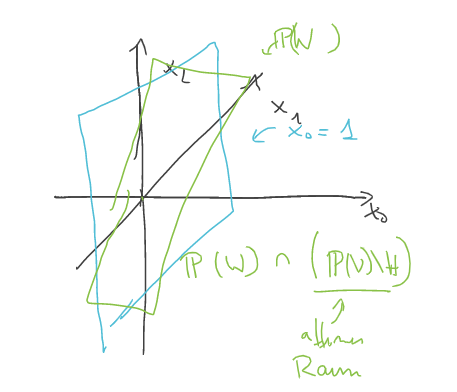
\includegraphics[width=0.5\linewidth]{beliebige_einbettung_affiner_raum_in_projektiven_raum}
  \label{fig:beliebige_einbettung_affiner_raum_in_projektiven_raum}
\end{figure}
\begin{satz}\label{projektiver_raum_als_affiner_raum}
  Sei \( V \) ein \( K \)-Vektorraum und \( H\subseteq \projectionspace{V} \) eine Hyperebene. Setze \( X\definedas \projectionspace{V}\setminus H\). Dann gibt es einen \( K \)-Vektorraum \( T(X) \) und eine einfach transitive Gruppenoperation
  \begin{equation*}
    \tau\maps T(X)\to \bijections{X},
  \end{equation*}
  sodass \( (X,T(X),\tau) \) ein affiner Raum ist mitfolgenden Eigenschaften:
  \begin{eigenschaftenenumerate}
    \item\label{projektive_unterraeume_in_affine_unterraeume} Ist \( Z\in \projectionspace{V} \) ein projektiver Unterraum mit \( Z\not\subseteq H \). Dann ist \( Z\cap X\subseteq X \) ein affiner Unterraum von \( X \) und es gilt
    \begin{align*}
      \affindim{Z\cap X}=\projectivedim-{Z}\\
      \projectivedim{}{Z\cap H}=\projectivedim-{Z}-1.
    \end{align*}
    Die Abbildung
    \begin{equation*}
      \begin{split}
      \alpha\maps \Set{\parbox{0.4\textwidth}{proj.\ Unterräume von \( \projectionspace-{(V)} \), die nicht in \( H \) enthalten sind}}&\to \Set{\parbox{0.4\textwidth}{nicht-leere affine Unterräume von \( X \)}}\\
      Z&\mapsto Z\cap X
      \end{split}
    \end{equation*}
    ist bijektiv.
    \item \label{projektivitaeten_in_affinitaeten} Sei \( f\maps \projectionspace{V}\to \projectionspace{V} \) eine Projektivität mit \( f(H)=H \). Dann ist \( \evaluateat{f}{X}\maps X\to X \) eine Affinität. Die Abbildung
    \begin{equation*}
      \begin{split}
        \beta\maps \Set{\text{Projektivitäten \( f \) von \( \projectionspace{V} \) mit \( f(H)=H \)}}&\to \Set{\text{Affinitäten von \( X \)}}\\
        f&\mapsto \evaluateat{f}{X}
      \end{split}
    \end{equation*}
    ist eine Bijektion.
  \end{eigenschaftenenumerate}
\end{satz}
\begin{proof}
  \begin{proofdescription}
    \item[Konstruktion des affinen Raumes \( (X,T(X),\tau) \)] Sei \( H=\projectionspace{W} \) mit \( W\subseteq V \) ein \( K \)-Vektorraum. Wähle \( v_0\in V\setminus W \) und definiere den affinen Unterraum
    \begin{equation*}
      X'\definedas V_0+W\subseteq V
    \end{equation*}
    mit \( (V,V,\explain{\text{Translation}}{\tau}) \) als affiner Raum.
    \begin{figure}[H]
      \centering
      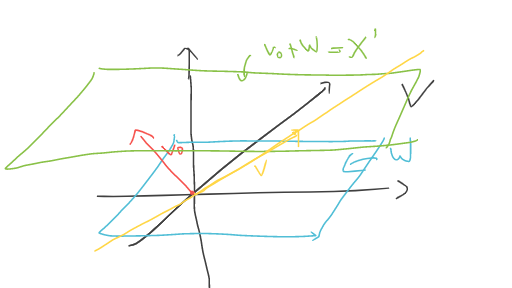
\includegraphics[width=0.5\linewidth]{affiner_raum_entsprechend_projektiver_hyperebene}
      \label{fig:affiner_raum_entsprechend_projektiver_hyperebene}
    \end{figure}
    Wir definieren eine Abbildung
    \begin{equation*}
      \begin{split}
        \sigma\maps X'&\to X\\
      X'\ni V&\mapsto K\cdot v.
      \end{split}
    \end{equation*}
    Für \( x\in X' \) ist \( K\cdot v\not\in \projectionspace{W}=H \), da \( v\in W \). Also ist \( \sigma\maps X'\to X \) eine wohldefinierte Abbildung. Wir zeigen, dass \( \sigma \) eine Bijektion ist.
    \begin{proofdescription}
      \item[\( \sigma \) ist injektiv:] Seien \( v,v'\in X' \) mit \( K\cdot v=Kv' \). Dann wären \( v \) und \( v' \) linear abhängig, aber \( X' \) enthält keine linear abhängigen Vektoren.
      \item[\( \sigma \) ist surjektiv] Sei \( p\in \projectionspace{V}\setminus H \) gegeben durch \( p=K\cdot v \) mit \( v\in V\setminus W \). \begin{behauptung*}
        Dann ist 
        \begin{equation*}
          p\cap X'\neq \emptyset.
        \end{equation*}
      \end{behauptung*} 
      Verwende die Dimensionsformel für affine Unterräume. Falls \( X'\cap p=\emptyset \), dann
      \begin{align*}
        \equalto{\affindim-{V}}{\affindim{X'\vee p}}&=\textcolor{LimeGreen}{\affindim-{X'}}+\textcolor{Goldenrod}{\affindim-{p}}-\dim{T(X')\cap T(p)}+1\\
        &=\textcolor{LimeGreen}{\affindim{V}-1}+\textcolor{Goldenrod}{1}-\affindim{\braceannotate{=\zeroset}{W\cap K\cdot v}}+1\\
        &=\affindim-{V}-0+1\quad \contra.
      \end{align*}
      Also ist \( p\cap X'\neq \emptyset \) und nach der Dimensionsformel für affine Unterräume folgt \( \anzahl{p\cap X'}=1 \), und
      \begin{equation*}
        p\cap X'\mapsto K\cdot(p\cap X')=\equalto{\sigma(p\cap X')}{p}.
      \end{equation*}
    \end{proofdescription}
    \begin{idee*}
      Verwende \( \sigma \) um die Struktur von \( X' \) als affinen Raum auf \( X \) zu übetragen.
    \end{idee*}
    \( X' \) ist ein affiner Raum \( (X',T(X'),\tilde{\tau}) \) mit \( T(X')=W \) und Gruppenoperation
    \begin{align*}
      \tilde{\tau}&\maps \begin{aligned}[t]
        W&\mapsto  \bijections{X'}\\
        w&\mapsto \tilde{\tau}_w
      \end{aligned}\\
      \tilde{\tau}_w&\maps \begin{aligned}[t]
        X&\to X\\
        x&\mapsto w+x
      \end{aligned}.
    \end{align*}
    Wir setzen \( T(X)=W \) und definieren eine Gruppenoperation
    \begin{equation*}
      \begin{split}
        \tau\maps W&\to \bijections{X}\\
        w&\mapsto \tau_w.
      \end{split}
    \end{equation*}
    durch
    \begin{equation*}
      \tau_{w(p)}\definedas \sigma\parens*{\tilde{\tau}_w\parens{\braceannotate{\in X'}{\inverse{\sigma}(p)}}}.
    \end{equation*}
    \begin{figure}[H]
      \centering
      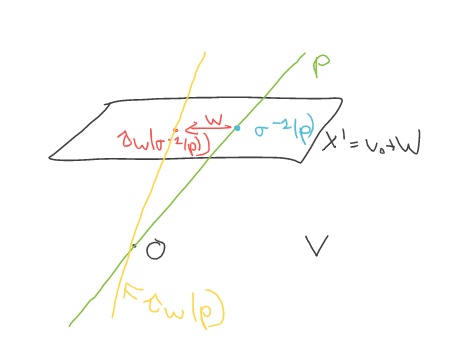
\includegraphics[width=0.5\linewidth]{gruppenoperation_auf_projektivem_raum_ohne_projektiver_hyperebene}
      \label{fig:gruppenoperation_auf_projektivem_raum_ohne_projektiver_hyperebene}
    \end{figure}
    Dann ist \( (X,T(X),\tau) \) affiner Raum und
    \begin{equation*}
      \sigma\maps X'\to X 
    \end{equation*}
    Affinität.
    \item[\ref{projektive_unterraeume_in_affine_unterraeume}] Sei \( Z=\projectionspace{U} \) projektiver Unterraum von \( \projectionspace{V} \) mit \( U\untervektorraum V \) \( K \)-Untervektorraum und \( Z\not\subseteq H \), also \( Z\cap X\neq \emptyset \). Dann ist \( \underrelate{\vertrelation{\subseteq}}{V}{X'}\cap  \underrelate{\vertrelation{\subseteq}}{V}{U} \) affiner Unterraum von \( X' \) und
    \begin{equation*}
      Z\cap X=\sigma(X'\cap U)
    \end{equation*}
    affiner Unterraum von \( X \).
    \minisec{Berechnung von \( \affindim{Z\cap X} \) und \( \projectivedim{Z\cap H} \)} Sei \( \dim-{V}=n+1 \). Es ist \( X'\cap U\neq \emptyset \), also folgt von der affinen Dimensionsformel
    \begin{equation*}
      n+1=\affindim{U\vee X'}=\affindim-{U}+\braceannotate{=n}{\affindim-{n}}-\affindim{U\cap X'}.
    \end{equation*}
    Es folgt
    \begin{equation*}
      \affindim{U\cap X'}=\affindim-{U}-1
    \end{equation*}
    und
    \begin{equation*}
      \affindim{Z\cap X}=\affindim{\sigma(X'\cap U)}=\affindim-{U}-1=\explain{\text{als projektiver Raum}}{\projectivedim-{Z}}.
    \end{equation*}
    Aus  \( Z\not\subseteq H \) folgt \( Z\vee H=\projectionspace{V} \). Aus der projektiven Dimensionsformel folgt
    \begin{equation*}
      n=\projectivedim-{Z\vee H}=\projectivedim-{Z}+\braceannotate{=n-1}{\projectivedim{H}}-\projectivedim-{Z\cap H},
    \end{equation*}
    also
    \begin{equation*}
      \projectivedim-{Z\cap H}=\projectivedim-{Z}-1.
    \end{equation*}
    Wir wollen zeigen, das 
    \begin{equation*}
      \begin{split}
      \alpha\maps \Set{\parbox{0.4\textwidth}{proj.\ Unterräume von \( \projectionspace-{(V)} \), die nicht in \( H \) enthalten sind}}&\to \Set{\parbox{0.4\textwidth}{nicht-leere affine Unterräume von \( X \)}}\\
      Z&\mapsto Z\cap X
      \end{split}
    \end{equation*}
    eine Bijektion ist. Wir konstruieren dazu eine Umkehrabbildung \( \alpha' \). Sei \( \emptyset \neq Y\subseteq X \) affiner Unterraum und
    \begin{equation*}
      Y'\definedas \inverse{\sigma}(Y).
    \end{equation*}
    Dann ist \( Y' \) affiner Unterraum von \( X' \) und
    \begin{equation*}
      T(Y')\subseteq  T(X')=W
    \end{equation*}
    Untervektorraum. Sei \( v\in Y' \). Definiere
    \begin{equation*}
      U\definedas K\cdot v+T(Y').
    \end{equation*}
    Wegen \( v\in Y'\subseteq X' \) gilt sogar \( v\not\in W \) und
    \begin{equation*}
      U=K\cdot v\oplus T(Y').
    \end{equation*}
    \begin{figure}[H]
      \centering
      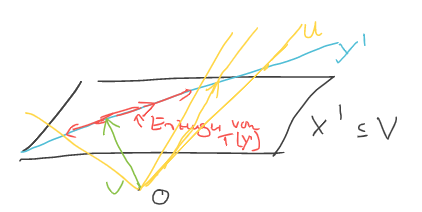
\includegraphics[width=0.5\linewidth]{affiner_unterraum_entsprechend_projektivem_unterraum.png}
      \label{fig:affiner_unterraum_entsprechend_projektivem_unterraum.png}
    \end{figure}
    Sei \( \overline{Y}\definedas \projectionspace{U} \). Dann ist \( \overline{Y} \) projektiver Unterraum von \( \projectionspace{V} \). Sei
    \begin{equation*}
      \alpha'(Y)\definedas \overline{Y}.
    \end{equation*}
    Dann ist \( \alpha' \) Umkehrabbildung zu \( \alpha \), denn
    \begin{equation*}
      \alpha'(\alpha(Z))=Z\cap X=Z
    \end{equation*}
    und
    \begin{align*}
      \alpha(\alpha'(Y))=\overline{Y}\cap X=Y.
    \end{align*}
    \item[\ref{projektivitaeten_in_affinitaeten}] Sei \( f\maps \projectionspace{V}\to \projectionspace{V} \) Projektivität mit \( f=\projectionmap{F} \) für einen Isomorphismus \( F\maps V\to V \). Wir nehmen an, dass \( f(H)=H \), also \( F(W)=W \) nach Skalieren von \( F \) können wir annehmen, dass 
    \begin{equation*}
      F(v_0)\in X'.
    \end{equation*}
    \begin{figure}[H]
      \centering
      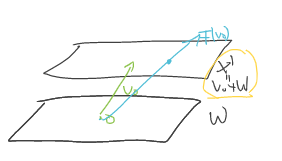
\includegraphics[width=0.5\linewidth]{projektiv_und_afin_skalieren_bringt_v_0_ins_bild_von_F} % dieser Name ist quatsch
      \label{fig:projektiv_und_afin_skalieren_bringt_v_0_ins_bild_von_F}
    \end{figure}
    Es gilt dann
    \begin{equation*}
      F(X')=X'.
    \end{equation*}
    \begin{behauptung*}
      \( \evaluateat{F}{X'}\maps X'\to X' \) ist Affinität mit zugehöriger linearen AB
      Abbildung
      \begin{equation*}
        \evaluateat{F}{W}\maps \equalto{W}{T(X')}\to T(X').
      \end{equation*}
    \end{behauptung*}
    \emph{denn:} sind \( x_1,x_2\in X'\subseteq V \), dann
    \begin{align*}
      \vv{\evaluateat{F}{x'}(x_1)\evaluateat{F}{X'}(x_2)}&=\vv{F(x_1)F(x_2)}\\
      &=F(x_2)-F(x_1)\\
      &=F(x_2-x_1)\\
      &=F(\vv{x_1 x_2})\quad \checkmark
    \end{align*}
    und \( F \) ist bijektiv.

    Damit ist auch
    \begin{equation*}
      \evaluateat{f}{X}\maps X\to X
    \end{equation*}
    Affinität, denn
    \begin{equation*}
      \evaluateat{f}{X}=\sigma \circ \evaluateat{F}{x'}\circ \inverse{\sigma}.
    \end{equation*}
    \file{Afiine projektive Geometrie Teil 2}
    Wir müssen nun zeigen, dass die Abbildung
    \begin{equation*}
      \begin{split}
        \beta\maps \Set{\text{Projektivitäten \( f \) von \( \projectionspace{V} \) mit \( f(H)=H \)}}&\to \Set{\text{Affinitäten von \( X \)}}\\
        f&\mapsto \evaluateat{f}{X}
      \end{split}
    \end{equation*}
    eine Bijektion ist. Wir konstruieren eine Umkehrabbildung \( \beta' \). Sei \( g\maps X\to X \) Affinität, mit zugehöriger linearer Abbildung
    \begin{equation*}
      G\maps \equalto{T(X)}{W}\to \equalto{T(X)}{W}.
    \end{equation*}
    Wegen \( v_0\not\in W \) gilt 
    \begin{equation*}
      V=W\oplus K\cdot v_0.
    \end{equation*}
    Wir definieren einen Isomorphismus \( \tilde{G}\maps V\to V \) durch
    \begin{align*}
      \evaluateat{\tilde{G}}{W}&=G\\
      \tilde{G}(v_0)&=\inverse{\sigma}(g(\sigma(v_0)))
    \end{align*}
    und setzen 
    \( \overline{g}=\projectionmap{\tilde{G}} \).
    Dann gilt 
    \( \evaluateat{\overline{g}}{X}=g \),
    \( \overline{g}(H)=H \)
     und 
     \( \overline{\evaluateat{f}{X}}=f \),
      also ist 
      \( \inverse{\beta}(g)=\overline{\beta} \) 
      invers zu \( \beta \).
  \end{proofdescription}  
\end{proof}
\begin{bemerkung*}[ohne Beweis]
  Im \thref{projektiver_raum_als_affiner_raum} haben wir gezeigt, wie man das Komplement
  \begin{equation*}
    \projectionspace{V}\setminus H\quad H\subseteq \projectionspace{V}\text{ Hyperebene}
  \end{equation*}
  als affinen Raum verstehen kann. Man kann auch zeigen, dass jeder affine Raum Resultat solch einer Konstruktion ist. \Dh für einen beliebigen affinen \( (X,T(X),\tau) \) gibt es einen projektiven Raum \( \projectionspace{V} \), eine Hyperebene \( H\subseteq \projectionspace{V} \) und eine Affinität
  \begin{equation*}
    X\to \projectionspace{V}\setminus H,
  \end{equation*}
  wobei \( \projectionspace{V}\setminus H \) wie in \thref{projektiver_raum_als_affiner_raum} als affiner Raum verstanden wird. 
\end{bemerkung*}